% This LaTeX file contains your written lab questions.  You may answer these
% questions just by inserting your answer into this document.
%
% If you're unfamiliar with LaTeX, see the document LearningLaTeX.tex in this
% same directory.  It contains a brief explanation and a few snippets of LaTeX
% code to get you started; in fact, it should have everything you need to
% complete this assignment.
%
% Also see the example file in examples/week-04/bigO.tex
\documentclass{article}

\usepackage{amsmath}
\usepackage{amssymb}
\usepackage{amsthm}
\usepackage{graphicx}

\begin{document}

    \section{QuickSort}

    See the source code file \texttt{quickSort.cpp} and the tests given in
    \texttt{tests.cpp}.

    \section{Big-O Proofs}

    \vspace{2mm}
    \noindent {\large\textbf{Problem 1.}} Show that $5n^3+n^2+4$ is $O(n^3)$.

    % Write your proof of the above statement here.
    $c = 10$

    $n_{0} = 1$
    
    for $n \ge 1 = n_{0}$

    $5n^{3}+n^{2}+4 \le 10n^{3}$

    $5n^{3}+n^{2}+4 \le 5n^{3}+n^{3}+4n^{3} \le 10n^{3}$  since $n \ge 1$

    \vspace{1cm}
    \noindent {\large\textbf{Problem 2.}} Show that $2n^4-3n^2+n$ is $O(n^4)$.

    % Write your proof of the above statement here.

    $c = 3$

    $n_{0} = 1$

    for $n \ge 1 = n_{0}$

    $2n^{4}-3n^{2}+n \le 3n^{4}$

    $2n^{4}-3n^{2}+n \le 2n^{4}+n^{4} \le 3n^{4}$  since $n \ge 1$

    \vspace{1cm}
    \section{Mystery Functions}

    % Give your explanation of each of the mystery functions here.

    fnA (f3) is linear $O(n)$ because for any $n$ the number of steps will be $n/2$ 
    where 2 is a constant that does not affect the big O. fnA is f3, because fnA 
    is the fastest function, and the slope of f3 was lower than all the others.
    \vspace{5mm}

    fnB (f5) is quadratic $O(n^{2})$ because for any $n$ the amount of steps 
    taken will be $n^{2}$. fnB is f5, becuse fnB is the third slowest function, 
    after fnD, which is O$(n^{4})$, and fnF, which is O$(n^{3})$.
    \vspace{5mm}

    fnC (f4) is $O(nlogn)$ because the outer for loop runs $n$ times. And each time 
    the while loop runs the number of steps will be cut in half, thus making it $logn$.
    fnC is f4 because the $O(nlogn)$ function is slower than the two linear functions, 
    fnA and fnE (as shown below), and is faster than the other functions, which f4 is.
    \vspace{5mm}

    \begin{center}
        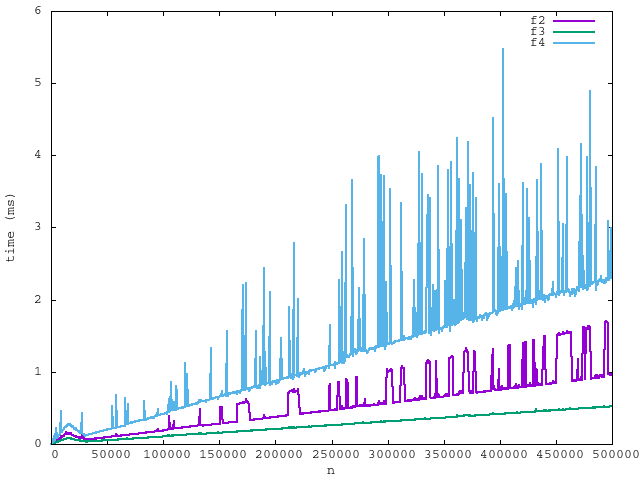
\includegraphics[width=0.8\textwidth]{f2_f3_f3_10_50000}
    \end{center}

    fnD (f6) is $O(n^{4})$ because for any $n$ the amount of steps taken 
    for the function to finish is $(n*n)(n*n)$. fnD is f6 because fnD is the slowest
    function, and f6 has the highest slope.
    \vspace{5mm}

    fnE (f2) is linear $O(n)$ beacuse for any $n$ the number of steps will be $4n$ 
    where 4 is a constant that does not affect the big O. fnC is f4 because fnE is 
    the second fastest function, after fnA (which is also linear, but has a smaller 
    constant), and f4 has the second lowest slope.
    \vspace{5mm}

    fnF (f1) is $O(n^{3})$ because for any $n$ the amount of steps taken 
    for the function to finish is n-cubed. fnF is f1, because it is the second 
    slowest function after fnD, which is $O(n^{4})$, and f1 has the second highest 
    slope (see figure below).
    
    \begin{center}
        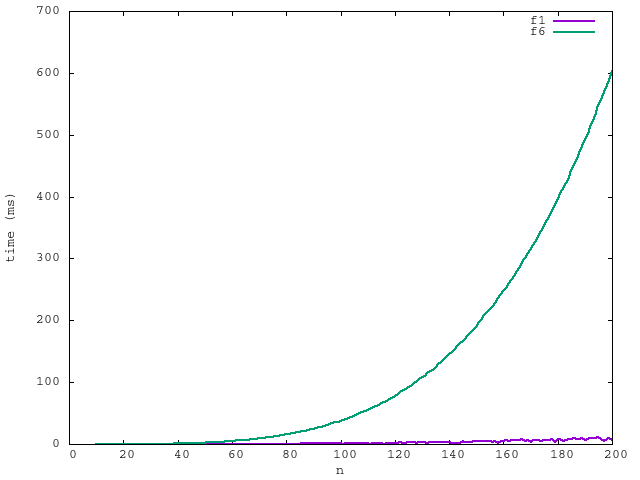
\includegraphics[width=0.8\textwidth]{f1f6}
    \end{center}

    % After your explanations, list the mystery functions A-E in sorted
    % order from fastest to slowest.  This will help you as you try
    % to determine the mappings in the empirical experiments.

    Functions in sorted order from fastest to slowest:

    fnA

    fnE

    fnC

    fnB

    fnF

    fnD
    
    % To include a png file, use the \includegraphics command
    % e.g. if you have a file 56.png comparing functions 5 and 6,
    % include it with the following command
    % \begin{center}
    %   \includegraphics[width=0.8\textwidth]{56}
    % \end{center}
\end{document}
